\documentclass[11pt]{report} 

\usepackage{projectreport}
\usepackage{pythonhighlight}
\usepackage{subcaption}
\usepackage{xcolor}
\definecolor{ForestGreen}{RGB}{34,139,34}

\newcounter{tmp}

\newcommand{\name}{Enrico Zorzi}
\newcommand{\course}{Project of automated reasoning}
\newcommand{\projecttitle}{Implementation of the congruence closure algorithm}
\newcommand{\submissiondate}{June 2023}

\begin{document}

\maketitle

\chapter*{Introduction}
\section*{Project Description}
In this project, i have implemented a solver based on the congruence closure decision algorithm. The solver is capable of analyzing an SMT-LIB formula or a plain formula, constructing a CC-DAG graph, and solving the satisfiability of the formula. The code is written in Python language utilizing various libraries, including NetworkX, Matplotlib, and PySMT.


\section*{Code Structure}
The code is divided in 3 sections,parse,CC-DAG and main function.

\subsection*{Parsing the Formula}
\begin{itemize}
    \item \texttt{parse\_formula(formula, dag)}: This function is responsible for analyzing the formula and extracting the necessary information to construct the CC-DAG graph.
    
    It uses regular expressions to separate subformulas, handle equalities and inequalities, and identify the nodes present in the formula.
    
    \item \texttt{translate\_string(formula)}: This function translates the formula into a string format that can be understood by the CC-DAG solver, removing unnecessary characters and rewriting certain operators.
    \item \texttt{update\_eq\_ineq(equalities, inequalities, nodes)}: This function updates the equality and inequality information based on the list of visited nodes.
    
\end{itemize}


\subsubsection*{Constructing the CC-DAG Graph}
\begin{itemize}
    \item \texttt{create\_graph(dag, nodes)}: This function constructs the CC-DAG graph from the list of visited nodes.It assigns a unique ID to each node and establishes the dependency relationships between nodes. Additionally, it handles function nodes and their arguments.
    \item \texttt{visit(node, nodes)}: This function adds a node to the list of visited nodes.
    \item \texttt{recursive\_visit(node, nodes)}: This function performs a recursive visit of the nodes, handling cases of function nodes and breaking down their arguments.
    \item \texttt{sub\_visit(node, nodes)}: This function performs a visit of secondary nodes within a function node, handling nested node cases and removing redundant information.
    \item \texttt{visualize\_dag(dag)}: This function visualizes the CC-DAG graph using the Matplotlib and NetworkX libraries.
\end{itemize}


\subsection*{CC\_DAG Class}
The CC\_DAG class represents the CC-DAG solver and contains methods for solving the SMT-LIB formula using the CC-DAG algorithm.
\begin{itemize}
    \item \texttt{CC\_DAG}: The constructor of the CC\_DAG class initializes the necessary data structures and variables used in the CC-DAG algorithm.

    
    \item \texttt{solve(formula)}: This method checks the satisfiability of the formula by examining the CC-DAG graph. It iterates over all the inequalities in the formula and checks if the nodes representing their terms belong to different equivalence classes. If an inequality is violated, it returns False.
    
    \item \texttt{find(node)}: This method finds the representative node of the given node. It recursively traverses the parent pointers until it reaches the representative node and updates the parent pointers along the path to directly point to the representative.
    
    
    \item \texttt{union(id1, id2)}: It uses the heuristic to optimize the union operation by always attaching the node with the lower rank to the one with the higher rank.
    
    \item \texttt{congruent(id1, id2)}: This method checks if two nodes are congruent by comparing their representative nodes.
    \begin{lstlisting}[style=pythoncode]
    def congruent(self, id1, id2):
    n1 = self.NODE(id1)
    n2 = self.NODE(id2)
    if (len(n1["args"]) == len(n2["args"])):
        for i in range(len(n1["args"])):
            val1 = self.find(n1["args"][i])
            val2 = self.find(n2["args"][i])
            if val1 != val2:
                return False
        return True
    else:
        return False
    \end{lstlisting}
    
    \item \texttt{merge(id1, id2)}: This method merges the equivalence classes of two nodes by making one node the parent of the other. 
    
    \begin{lstlisting}[style=pythoncode]
    def merge(self, id1, id2):
        a1 = self.find(id1)
        a2 = self.find(id2)
        if a1 != a2:
            pi1 = self.ccpar(id1)
            pi2 = self.ccpar(id2)
            self.union(id1, id2)
            for t1, t2 in list(product(pi1, pi2)):
                if self.find(t1)!=self.find(t2) and self.congruent(t1, t2):
                    self.merge(t1, t2)
            return True
        else:
            return False
    \end{lstlisting}
    
    \item \texttt{ccpar(id)}: This method returns the parent of the given node.

\end{itemize}
\newpage
\section*{Main Function}
The main function of the code is responsible for reading the input formula from a file, constructing the CC-DAG graph, and solving the satisfiability of the formula. It uses the \texttt{parse\_formula} function to extract the necessary information from the formula and the \texttt{create\_graph} function to construct the CC-DAG graph. Finally, it uses the \texttt{solve} method of the CC\_DAG class to solve the satisfiability of the formula.
The main part of the code is shown below:
\begin{enumerate}
    \item Import necessary libraries and modules.
    
    \item If the script name is a \texttt{.smt2} file and exists, perform the following steps:
    \begin{enumerate}
        \item Start the timer.
        
        \item Use the \texttt{SmtLibParser} to parse the SMT-LIB script.
        
        \item Translate the formula to a string and remove unnecessary characters.
        
        \item Initialize a \texttt{CC\_DAG}. object
        
        \item Parse the formula and create a list of nodes.
        
        \item Sort the list of nodes in descending order of length.
        
        \item Create a graph using the \texttt{CC\_DAG} object and the list of nodes.
        
        \item Update the equalities and inequalities based on the list of nodes.
        
        \item Solve the formula using the \texttt{CC\_DAG} object and print the result.
        
        \item Stop the timer and print the elapsed time.
    \end{enumerate}
    
    \item If the script name is a \texttt{.txt} file and exists, perform the following steps:
    \begin{enumerate}
        \item Start the timer.
        
        \item Read the script file line by line.
        
        \item If a line contains "or", split the line by "or" and process each sub-formula separately.
        
        \item For each sub-formula, create a new \texttt{CC\_DAG} object, parse the sub-formula, create a list of nodes, sort the nodes, create a graph, update the equalities and inequalities, and solve the sub-formula.
        
        \item If a line does not contain "or", create a new \texttt{CC\_DAG} object, parse the formula, create a list of nodes, sort the nodes, create a graph, update the equalities and inequalities, and solve the formula.
        
        \item Print the result for each formula/sub-formula.
        
        \item Stop the timer and print the elapsed time.
    \end{enumerate}
\end{enumerate}
\section*{Use the Solver}
To use the solver, provide a .txt or .smt2 file as input to the \texttt{main} function. The solver will execute the CC-DAG algorithm on the formula and return the satisfiability result. 
Additionally, you can visualize the generated CC-DAG graph using the \texttt{visualize\_dag} function.

N.B. only the .txt can resolve formulas with "or" statements. 

\section*{Variants implemented}
\subsection*{Forbidden List}
The forbidden list is implemented by adding the inequalities to a set and checking if the pair of nodes to be merged is in the set. If the pair is in the set, the algorithm returns UNSAT.
\subsubsection*{Code implementation}
\begin{lstlisting}[style=pythoncode]
    def solve(self):
        forbiddenMerges = set()  # set of forbidden list

        for pair in self.inequalities:
            firstId, secondId = pair
            # add to forbidden list
            forbiddenMerges.add((firstId, secondId)) 

        for pair in self.equalities:
            firstId, secondId = pair
            firstId_find = self.find(firstId) 
            secondId_find= self.find(secondId)
            # check if pair is in forbidden list
            if (firstId_find, secondId_find) in forbiddenMerges: 
                return "UNSAT"
            self.merge(firstId, secondId)

        for pair in self.inequalities:
            firstId, secondId = pair
            if self.find(firstId) == self.find(secondId):
                return "UNSAT"
        return "SAT"
\end{lstlisting}



\subsection*{Non arbitrary choice of representative in union} 
The non arbitrary choice of representative in union is implemented by using the heuristic of attaching the node with the lower rank to the one with the higher rank. This is done by comparing the length of the equivalence classes of the two nodes and attaching the node with the lower length to the one with the higher length.
\subsubsection*{Code implementation}
\begin{lstlisting}[style=pythoncode]
    def union(self, id1, id2):
        n1 = self.NODE(self.find(id1))
        n2 = self.NODE(self.find(id2))
        # Compare the size of the ccpar sets
        if len(n1["ccpar"]) > len(n2["ccpar"]): 
            n2["find"] = n1["find"]
            n1["ccpar"].update(n2["ccpar"])
            n2["ccpar"] = set()
        else:
            n1["find"] = n2["find"]
            n2["ccpar"].update(n1["ccpar"])
            n1["ccpar"] = set()

\end{lstlisting}
\newpage
\section*{Data}
I take the .smt2 from the SMT-LIB-benchmarks/QF\_UF/-/tree/master/TypeSafe repository. 

The .txt file contains some formulas taken from book (The Calculus of Computation by Bradley and Manna) and other formulas created by me.

\subsection*{How to add more data}
To add more data, simply add the .smt2 or .txt file to /Test directory.
\subsubsection*{Format}
The .txt file must be in the following format:
\begin{lstlisting}[style=pythoncode]
    f(f(f(a))) = f(a) and f(f(a)) = a and f(a) != a
    f(x) = f(y) and x != y
    f(f(a))=f(b)&f(f(a))!=f(b)
    f(a, b) = a and f(f(a, b), b) != a
\end{lstlisting}
Only one formula per line, the function name indicated by "f" aand the variables should be separated by ",".

The formula with or statement should be in the following format:
\begin{lstlisting}[style=pythoncode]
    f(f(a))=f(b)&f(f(a))!=f(b) or f(f(a))=f(b)&f(f(a))!=f(b)
\end{lstlisting}

"or" statement is used to separate the sub-formulas.



\section*{Time Benchmark}
To measure the execution time of the solver, i conduct a benchmark on a set file. The time taken to solve each file is recorded below:
\begin{center}
\begin{tabular}{|c|c|}
\hline
\textbf{File} & \textbf{Execution Time (seconds)} \\
\hline
test1.smt2 & 0.017 \\
test2.smt2 & 0.022 \\
test3.smt2 & 0.013 \\
test4.smt2 & 0.015 \\
test5.smt2 & 0.014 \\
test.txt(8 formulas) & 0.044 \\

\hline
\end{tabular}
\end{center}
    
\newpage
\section*{Visualize Graph of .txt file}

\begin{figure}[h]

    \begin{subfigure}{0.5\textwidth}
        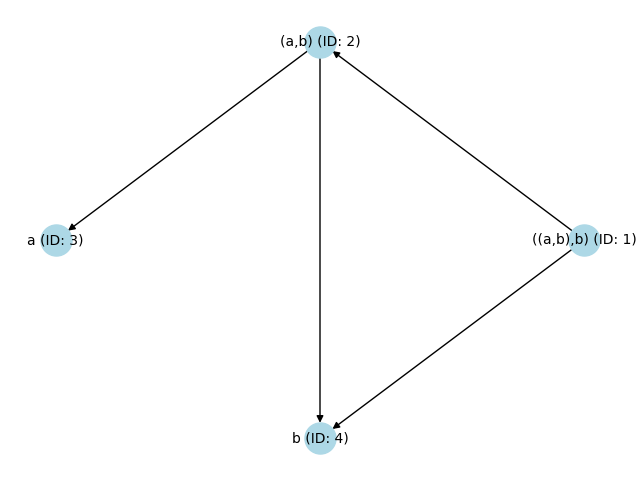
\includegraphics[width=0.9\linewidth, height=5.5cm]{graph/(a, b) = a and ((a, b), b) != a.png} 
        \caption*{(a, b) = a and ((a, b), b) != a \color{red}\# UNSAT }
        \label{fig:subim1}
        \end{subfigure}
    \begin{subfigure}{0.5\textwidth}
        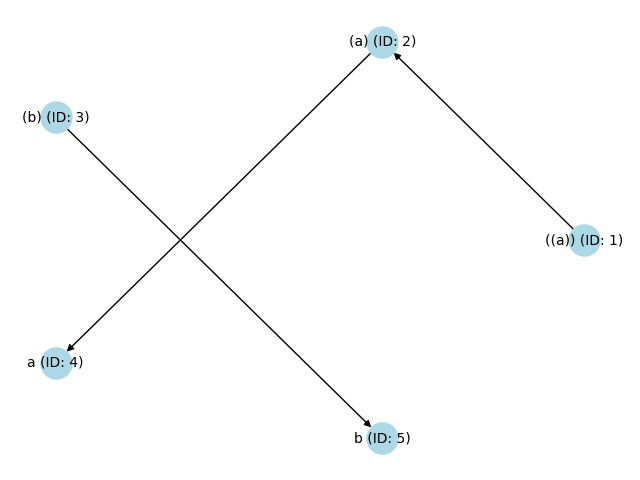
\includegraphics[width=0.9\linewidth, height=5.5cm]{graph/((a))=(b)&((a))!=(b).png} 
        \caption*{((a))=(b)\&((a))!=(b) \color{red}\# UNSAT}
        \label{fig:subim2}
        \end{subfigure}
    \begin{subfigure}{0.5\textwidth}
        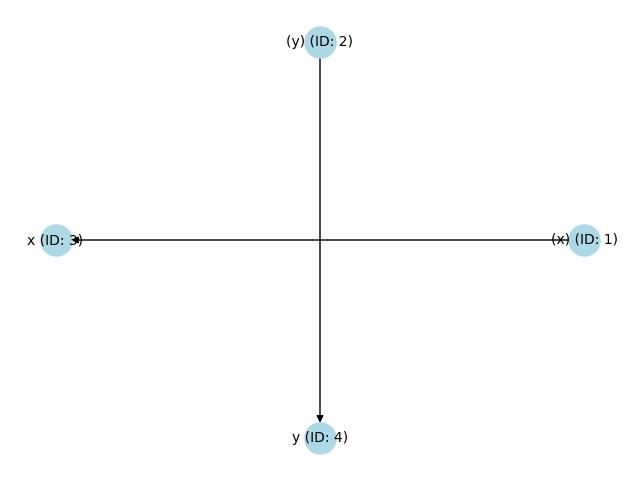
\includegraphics[width=0.9\linewidth, height=5.5cm]{graph/(x) = (y) and x != y.png}
        \caption*{(x) = (y) and x != y \color{ForestGreen}\# SAT}
        \label{fig:subim3}
        \end{subfigure}
    \begin{subfigure}{0.5\textwidth}
        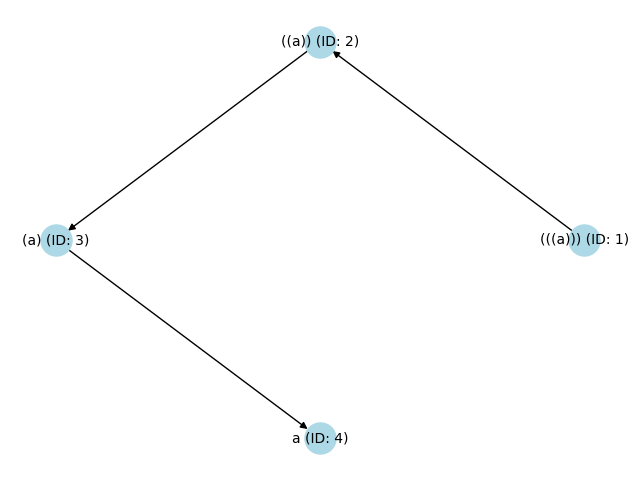
\includegraphics[width=0.9\linewidth, height=5.5cm]{graph/(((a))) = (a) and ((a)) = a and (a) != a.png}
        \caption*{(((a))) = (a) and ((a)) = a and (a) != a \color{ForestGreen}\# SAT}
        \label{fig:subim4}
        \end{subfigure}
    \begin{subfigure}{0.5\textwidth}
        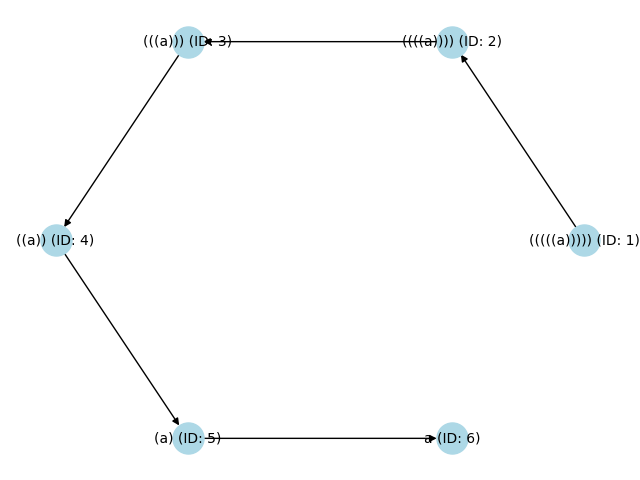
\includegraphics[width=0.9\linewidth, height=5.5cm]{graph/(((a))) = a and (((((a))))) = a and (a) != a.png}
        \caption*{(((a))) = a and (((((a))))) = a and (a) != a \color{red}\# UNSAT}
        \label{fig:subim5}
        \end{subfigure}
    \label{fig:image2}
    \end{figure}

\end{document}